% Weak Scalability Design : Keep Pipeline of Ensembles to show barrier needed in S5 and S6
% Performance, generality with weak scaling (agnostic to kernel)
% Added functionality (do not speak about binding adaptivity to performance or generality)
% In use case: add in why TIES is challenging, and why adaptivity is challenging

% ---------------------------------------------------------------------------
\subsection{Experiment Setup}\label{ssec:exp_design}

We perform experiments to characterize the overheads of HTBAC, its runtime
system and the weak and strong scaling performance on NCSA Blue Waters and 
ORNL Titan. 

\begin{table*}
    \caption{Parameters of scalability experiments.}\label{tab:experiments}
    \centering
    \resizebox{\textwidth}{!}{
    \begin{tabular}{l            % Experiment ID
                    l            % CI
                    l            % protocol type
                    l            % number of protocols
                    l            % total cores
                    l            % executable
                    }
    %
    \toprule
    %
    \B{ID}                            &  % Experiment ID
    \B{Computing Infrastructure (CI)} &  % CI
    \B{Protocol(s)}                   &  % protocol type
    \B{No. Protocol(s)}                    &  % number of protocols
    \B{Total Cores}                    &  % total cores
    \B{Executable}                          \\ % executable
    %
    \midrule
    %
    \B{1}                             &  % Experiment ID
    Blue Waters                       &  % CI
    ESMACS                            &  % protocol type
    (2, 4, 8, 16)                     &  % number of protocols
    1600, 3200, 6400                  &  % total cores
    NAMD-MPI                               \\ % executable
    %
    \B{2}                             &  % Experiment ID
    Titan                          &  % CI
    ESMACS                          &  % protocol type
    (16, 64, 128)                    &  % number of protocols
    6400, 25600, 51200              &  % total cores
    NAMD (non-MPI)                 \\ % executable
    % 
    \B{3}                             &  % Experiment ID
    Blue Waters                       &  % CI
    TIES                              &  % protocol type
    (2, 4, 8)                         &  % number of protocols
    4160, 8320, 16640                 &  % total cores
    NAMD-MPI                              \\ % executable
    %
    \B{4}                             &  % Experiment ID
    Titan                          &  % CI
    TIES                          &  % protocol type
    (8, 32, 64)                    &  % number of protocols
    16640, 66560, 133120              &  % total cores
    NAMD (non-MPI)                 \\ % executable
    %
    \B{5}                             &  % Experiment ID
    Blue Waters                       &  % CI
    ESMACS + TIES                     &  % protocol type
    (2, 4, 8)                    &  % number of protocols
    5280, 10560, 21120              &  % total cores
    NAMD-MPI                              \\ % executable
    %
    \B{6}                             &  % Experiment ID
    Blue Waters                          &  % CI
    TIES                          &  % protocol type
    (8, 8, 8)                    &  % number of protocols
    16640, 8320, 4160              &  % total cores
    NAMD-MPI                              \\ % executable
    %
    \B{7}                             &  % Experiment ID
    Blue Waters                          &  % CI
    ESMACS                          &  % protocol type
    (16, 16, 16)                    &  % number of protocols
    6400, 3200, 1600              &  % total cores
    NAMD-MPI                              \\ % executable
    %
    \bottomrule
    %
    \end{tabular}
    }
\up{}
\end{table*}

We show homogeneous and heterogeneous weak scalability of the protocols by
increasing the number of protocol instances while keeping the required number
of pipelines. By design of each protocol, an increase in the number of
instances means an increase in the number of pipelines. Experiment 1 measures
the weak scalability of HTBAC, EnTK and RP using multiple instances of the
ESMACS protocols on NCSA Blue Waters. Experiment 2 measures weak scaling
performance of ESMACS at higher scales, using ORNL Titan.
\mtnote{Would it be better to describe weak scaling in terms of solution
time, number of resources and problem size, as done in the following
paragraph?}

Experiments 3 and 4 repeat the same design as experiments 1 and 2 using the
TIES protocol instead of the ESMACS one. Experiment 5 uses both TIES and
ESMACS in the same run. By design of weak scaling, the ratio between the
number of pipelines and cores are kept constant. As the number of cores
(measure of resource) changes by a factor of 2, we introduce twice as many
protocol instances. In this way, the weak scaling property \mtnote{property
of? I would replace with: ``weak scaling provides insight\ldots''} provides
insight into the size of the workload that can be investigated in a given
amount of time.

Experiments 6 and 7 measure individual\mtnote{I am not sure I understand what
individual means in this context} strong scaling performance of ESMACS and
TIES on Blue Waters. We fix the number of protocols and vary the amount of
resources in order to produce generations \mtnote{The reader will struggle to
understand what `generations' means in this context.} of execution.
\mtnote{Two sizable paragraphs to describe weak scaling, four lines to
describe strong scaling? I would expand.}

Due to the NCSA and ORNL security policies, we performed the Blue Waters
experiments from a persistent virtual machine and the Titan ones from an ORNL
login node.
% as Blue Waters does not permit executing applications directly on the login
% node. The ORNL Titan experiments had instead to be performed from an ORNL
% login node.
We used HTBAC 0.1, EnTK 0.6, and RP 0.47 for all the experiments and
different versions of the NAMD MD engine, compiled according to the
capabilities of each environment and of NAMD itself. On Blue Waters we used
NAMD-MPI while on Titan a non-MPI, multi-core NAMD engine. On Titan we
compiled NAMD with CUDA for the ESMACS experiments, and with OpenMP for the
for TIES ones as NAMD does not support alchemical perturbations execution on
GPU.

We perform \mtnote{We used the preterite until now} all Blue Waters
experiments using the APRUN launch method \mtnote{does the reader know what
is a launch method?}, which has an upper limit of avg 436 concurrent task
execution \mtnote{how do we know this average?}. In order to continue
execution on higher scales \mtnote{Why do we need an higher scale?}, we
perform higher scales \mtnote{I am not sure what `performing higher scales'
means} on ORNL Titan, using the ORTE launch method \mtnote{Why don't we use
ORTE on BW? The reader will probably know that they are similar machines}.
The difference in platforms produces overheads \mtnote{Only overheads or also
different execution time of NAMD---seeing the differences described in the
previous paragraph} that can be captured by RTS \mtnote{does the reader know
what a RTS is?} and are shown \mtnote{careful with the use of `demonstrate',
especially in a scientific paper} in the figures \mtnote{which figures?} as
"APRUN overhead" and "ORTE overhead" \mtnote{LaTeX requires different
quotes}.

For tasks pertaining to $S1$ - $S4$ \mtnote{What are $S1$ and $S4$? LaTeX
wants double dash without space to indicate a range}, while the analysis
stage, $S5$ use AmberTools \mtnote{grammar: I am not able to parse this
sentence}. For both adaptive and nonadaptive experiments \mtnote{the reader
knows about Experiment 1-7, not about adaptive/nonadaptive ones}, the
minimization tasks of $S1$ are assigned 1000 steps, while the equilibration
tasks in $S2$ and $S3$ are assigned 5000 steps. In the nonadaptive
experiments, the production simulation tasks \mtnote{when/why a simulation
task is `production'? I am not sure I understand what that means} in $S4$ are
assigned 50,000 steps. For the adaptive experiments, each substage
\mtnote{What is a `substage'?} of $S4$ i.e. $S4.1$--$S4.4$ is assigned 50,000
steps.\mtnote{Why the difference is number of steps and why it is relevant?}

% HTBAC submits a resource request to EnTK, to which EnTK uses RP to acquire
% resources via a single pilot. Accordingly, we request the maximum number of
% cores required by the workload as the number of cores in a pilot.

For weak scaling performance of TIES \mtnote{I am not sure I understand this
sentence: For measuring the weak scaling performance of TIES?}, we use
between 4160 and 33280 cores as indicated in
Figure~\ref{fig:weak_scaling_TIES} because the NAMD executable used in all
tasks \mtnote{does the reader know what a task is in this context?} from
$S1$-$S4$ require \mtnote{grammar: requires} at least 32 cores per task
\mtnote{why?}. From our own scalability performance measurements of NAMD on
Blue Waters, we observe the ideal cores per task to be 16, however Blue
Waters does not permit running multiple MPI applications on the same node,
hence each NAMD task requires a full node to maintain concurrency.
\mtnote{This needs to go before previous sentence as it explains why we use
32 cores for each NAMD executable. Note: it is not true that NAMD `requires'
32 cores as stated above.}

For strong scaling performance, we fix the number of protocol instances to 8
instances \mtnote{why 8?} and vary the amount of resources as shown in
Figure~\ref{fig:strong_scaling_TIES}. \mtnote{Please expand indicating and
justifying the the chosen amount of resources. Experiments can be design in
many ways, we need not only to describe but also to justify why we choose a
specific design for our experiments.}

For the TIES protocol, each pipeline \mtnote{does the reader know what a
pipeline is?} consists of six stages \mtnote{simulation stages?}. Each of the
simulation stages contains a task for every unique ($\lambda$, replica)
combination \mtnote{does the reader understand this?}. In the non-adaptive
workflow \mtnote{we never used `workflow'. Previously we used non-adaptive
(written as `nonadaptive') experiment. Note that we did not introduce
adaptive/nonadaptive experiments} scenario, the first 11 $\lambda$ windows
\mtnote{does the reader know what a lambda window is?} consist of the
following values: $L$ is a vector with
\begin{flalign}
L &= \{ x_i: x_i\in[0,1]\; and\; x_{i+1} = x_i + \delta \}, where\ \delta\ is\ 0.1.
%&$$L=\{ x_i: x_i\in[0,1]\; and\; x_{i+1} = x_i + \delta \}$$%, where $\delta$ is $0.1$.
\end{flalign}

We append two additional values on both ends of $L$, completing 13 $\lambda$
windows. Each $\lambda$ window consists of five replicas. Therefore there are
a total of 65 tasks for every simulation stage \mtnote{depending on the
previous sections of the paper, this `therefore' may have to be better
explained to the reader}. The production simulations stage, $S4$ as described
in figure~\ref{fig:pst}\mtnote{missing figure} executes a 4 ns simulation
duration \mtnote{grammar: executes a simulation for 4 ns? a simulation with a
4 ns duration?}. The analysis stages of the protocol reduce the number of
tasks \mtnote{Why/how?}. The first analysis task consists of five tasks where
each task performs an aggregate analysis over all $\lambda$ windows for each
replica. The second analysis stage consists of one task that aggregates the
previous results and computes a single average across all replicas.

%----------------------------------------------------------------------------
\subsubsection{Scaling and Performance Characterization}

\mtnote{Is this meant to be a subsubsection?}

We first characterize the overheads of HTBAC and the runtime system. HTBAC
enables concurrent execution of multiple protocol \mtnote{what type of
protocols?} instances. The overhead of HTBAC depends \mtnote{mostly?} on the
number of protocol instances that need to be generated for an application.
% With each new protocol instance generated for an application, the HTBAC
% overhead grows to match the additional requirement of generating new
% protocols.
The total time to completion (TTC) \mtnote{of what?} can be expressed as
following: $TTC = TTX + T_{O}$ where \(TTX\) measures the execution duration
across all task, including file staging, MD kernel execution, pre- and
post-executables \mtnote{TTX should measure only the aggregated time spent
executing the tasks' executables. All the rest should be part of RP
overhead}; and $T_{O}$ the total overhead is \mtnote{grammar: I do not
understand the sentence after the `;'} given by the sum of the constituent
overheads: $$T_{O} = T_{O}\textsuperscript{HTBAC} +
T_{O}\textsuperscript{EnTK} + T_{O}\textsuperscript{RP}$$ \mtnote{As defined,
this formula seems to add twice part of the RP overheads.}

% In order to understand the contribution of the various events in HTBAC,
% termed as HTBAC overhead, to

%----------------------------------------------------------------------------
% \subsubsection{Weak Scaling Experiments}

We investigated the weak scalability properties for the TIES protocol by
growing the number of protocol instances while adhering to the required
number of pipelines. By design of each protocol, an increase in the number of
instances simply means an increase in the number of pipelines. The first weak
scalability experiment demonstrates the behavior of HTBAC, EnTK and RP using
the multiple instances of the TIES protocol. By design of weak scaling, the
ratio between the number of pipelines and cores are kept constant. As the
number of cores (measure of resource) changes by a factor of 2, we introduce
twice as many protocol instances. As designed, the weak scaling property
provides insight into the size of the workload that can be investigated in a
given amount of time.\mtnote{This paragraph is a copy of a previous
paragraph. See comments and iterations of the previous paragraph before
rewriting a new paragraph if needed.}

\begin{figure}
  \centering
    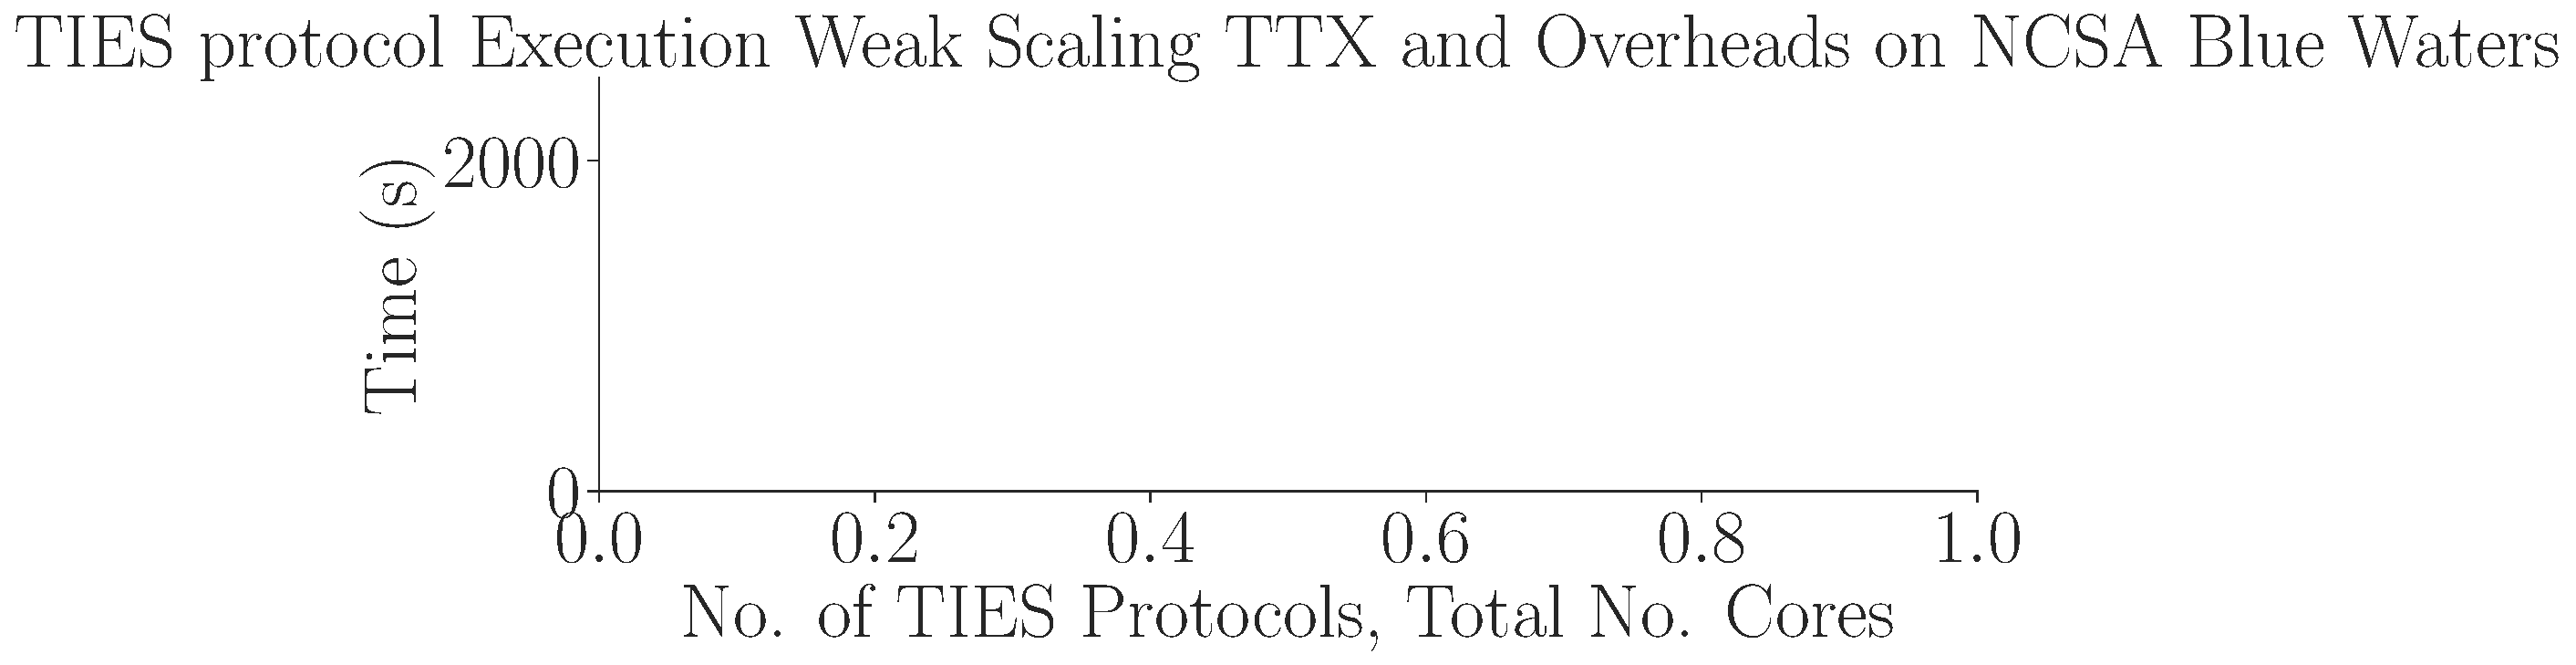
\includegraphics[width=\columnwidth]{figures/ties_ws_pseudo.pdf}
    \caption{Weak scaling properties of HTBAC. We investigate the weak
    scaling of HTBAC as the ratio of the number of protocol instances to
    resources is kept constant. Overheads of HTBAC (right), and runtime
    overhead (left) and \(TTX\) (left) for experimental configurations
    investigating the weak scaling of TIES. We ran X trials for each protocol
    instance configuration. Error bars in \(TTX\) in y-protocol runs are
    insignificant.}
\label{fig:weak_scaling_TIES}
\end{figure}

The second weak scalability experiment repeats the same experimental design
\mtnote{of what?}, replacing the TIES protocols \mtnote{should this be
`protocol'?} with TIES and ESMACS, respectively. \mtnote{This paragraph needs to be further expanded}

\begin{figure}
  \centering
    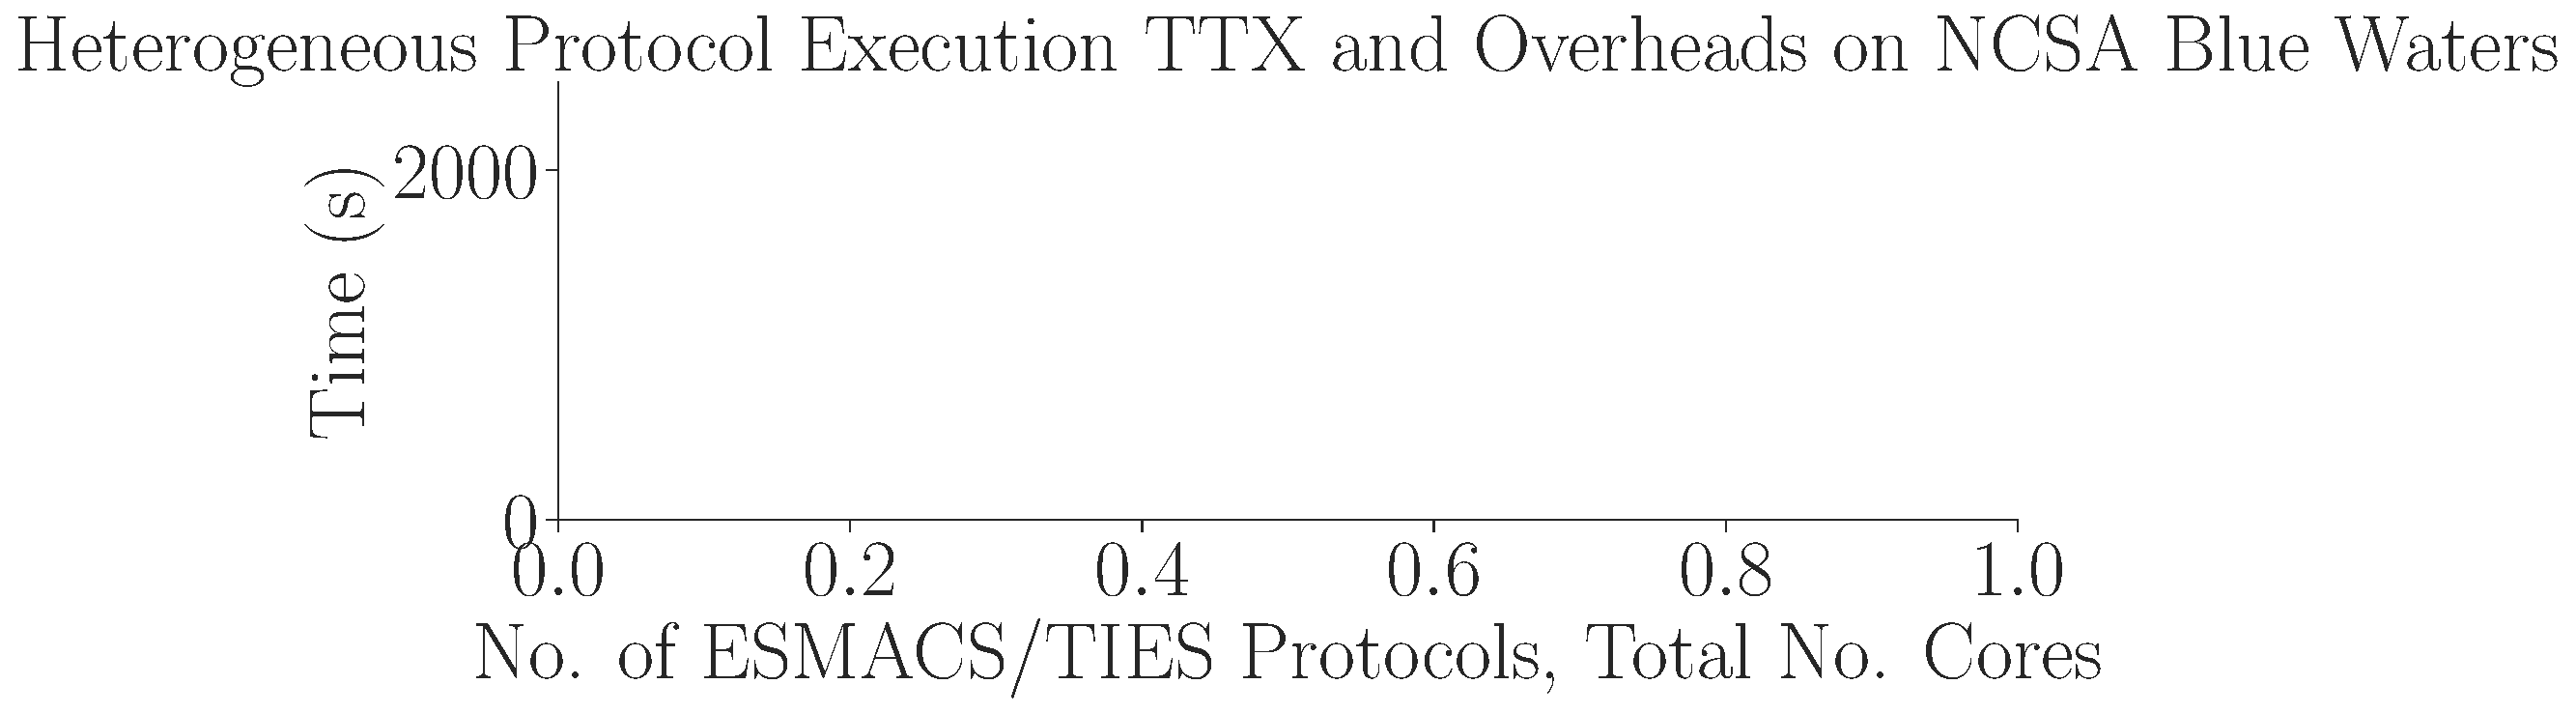
\includegraphics[width=\columnwidth]{figures/esmacs_ties_ws_pseudo.pdf}
    \caption{Weak scaling properties of HTBAC (right side). We investigate
    the weak scaling of HTBAC as the ratio of the number of ESMACS and TIES
    protocol instances to resources is kept constant. (Left) Overheads of
    HTBAC, and runtime overhead for experimental configurations. We ran X
    trials for each protocol instance configuration.}
\label{fig:weak_scaling_ESMACS_TIES}
\end{figure}

The HTBAC overhead shows a super linear increase as we grow the number of
protocol instances. However, the HTBAC overhead is a minimal contributor to
\(TTX\) \mtnote{Should this be TTC? HTBAC should contribute nothing to TTX.
If this should be TTX, then we should write about comparison between HTBAC
overhead and TTX}. The runtime overheads, mainly EnTK and RP, depend on the
number of tasks that need to be translated in-memory from a Python object to
a compute unit (CU) description \mtnote{This sentence is copied from a
previous paper we wrote: does the reader know what a CU is?}. As such, those
overheads are expected to grow proportionally to the number of tasks. EnTK
submits CU descriptions to a MongoDB used by RP. RP pilot pulls these
descriptions from the same database.\mtnote{I am not sure this is accurate}
% This pull operation occurs over a wide area networks, which introduces
% varying amounts of latency.
In addition, each stage constructed by EnTK maintains sequential barriers
\mtnote{Doe the reader know what a barrier is?}. RP remains dormant until
completion of the current tasks before staging the next tasks
\ref{fig:weak_scaling_ESMACS_TIES} \mtnote{This figure is about scaling
behavior, not about the mechanics of EnTK and RP here discussed.}

% The impact of the synchronization barriers increases with the number of CUs
% as seen in the 16 protocol instances data point in

Furthermore, an additional overhead, driven by the aprun \mtnote{Does the
reader know what aprun is? Also, I would use something like textttt to
identify the name of a command or executable} launch method, increases as we
approach a system limit on the number of permissible \mtnote{concurrent?}
aprun processes when scaling from 8 to 16 protocols, which translates to 520
and 1040 concurrent tasks, respectively \mtnote{this sentence does not read
well. I would refine it}. We account for the aprun failures in the \(TTX\)
\mtnote{this needs further explanation}. Together, the EnTK-enabled
synchronization barriers and aprun overhead failures \mtnote{until now, we
have implicitly assumed that our overheads are measured in time. Did we now
use also number of failures?} introduce delays in the scheduling of the CUs
and results in higher overheads \mtnote{Is this sentence circular? Overhead
increases contributing to increasing the overhead?}. Lastly, we notice that
each additional protocol instance contributes to roughly 55 additional
seconds in \(TTX\).\mtnote{All this needs to be clarified and expanded into
an actual discussion of the results.}

% ---------------------------------------------------------------------------
\subsubsection{Strong Scaling Experiments}

\mtnote{Should we have also a `Weak Scaling Experiments' header? Or maybe we
should change this one?}

Next we repeat the same design of the weak scalability experiments but
examine performance of strong scaling when fixing the number of pipelines and
varying the resources. The comparison between weak and strong scalability
shows the overhead introduced by load balancing and scheduling tasks in
multiple generations \mtnote{See previous comments about
terminology}\mtnote{I am not sure I understand: are we comparing overheads
when weak and strong scaling our applications/workflows or are we first
measuring the overheads when strong scaling and then comparing them to those
of weak scaling?}. As we scale the number of generation of concurrent tasks
executions, we half the resources allocated by the pilot \mtnote{this should
be explained in the experiment setup and design}.

\mtnote{General note. Experiments about weak and strong scaling show the
behavior of our software stack with one or more workflows/workloads. The
question these experiments answer to is: Given a workload/workflow, does this
software stack scale weakly and/or strongly? This is why, in the analysis of
our data, we look at the linearity (or lack of thereof) of our plots. The
analysis of the overhead(s) answer to a different question: What part of a
measure---e.g., time to completion---depends on the properties of an element
used to produce that measure---e.g., a component of our software stack?
Usually, the analysis of the overheads is used to explain why we observe lack
of scalability (weak or strong) as represented by a superlinearity in our
plots. The discussion of our experimental results should clearly distinguish
these questions and properly relate the study of scalability to that of
overheads. At the moment, our discussion does not do all this.}

Furthermore, as we scale the number of generations, the runtime overhead of
RP scales linearly. RP requires an amount of time to schedule tasks
proportional to the scale of execution. The main contributor to the increase
in overhead \mtnote{which one?} is derived \mtnote{I am not sure a
contributor is derived} by the time of resources inactivity while RP
schedules new tasks \mtnote{this is derived from another publication: we need
to reference the work we copy/paraphrase from}. As such, the overhead is
expected to grow proportionally to the number of concurrent tasks.

The RP overhead decomposes \mtnote{I do not think the overhead decomposes: Do
we measure the components of the overhead?} into events \mtnote{we use events
to record timestamps from which we derive durations that, once interpreted,
measure our overheads. I would avoid to mention events in this context.} that
capture the pilot and tasks lifespan. The pilot duration contains the time to
bootstrap and terminate the pilot. The task overheads contain the executor's
spawning of the task, folder staging preparation, and operating system task
spawning. \mtnote{We need to explain to the reader why all this is relevant
in this context.}

\begin{figure}
  \centering
    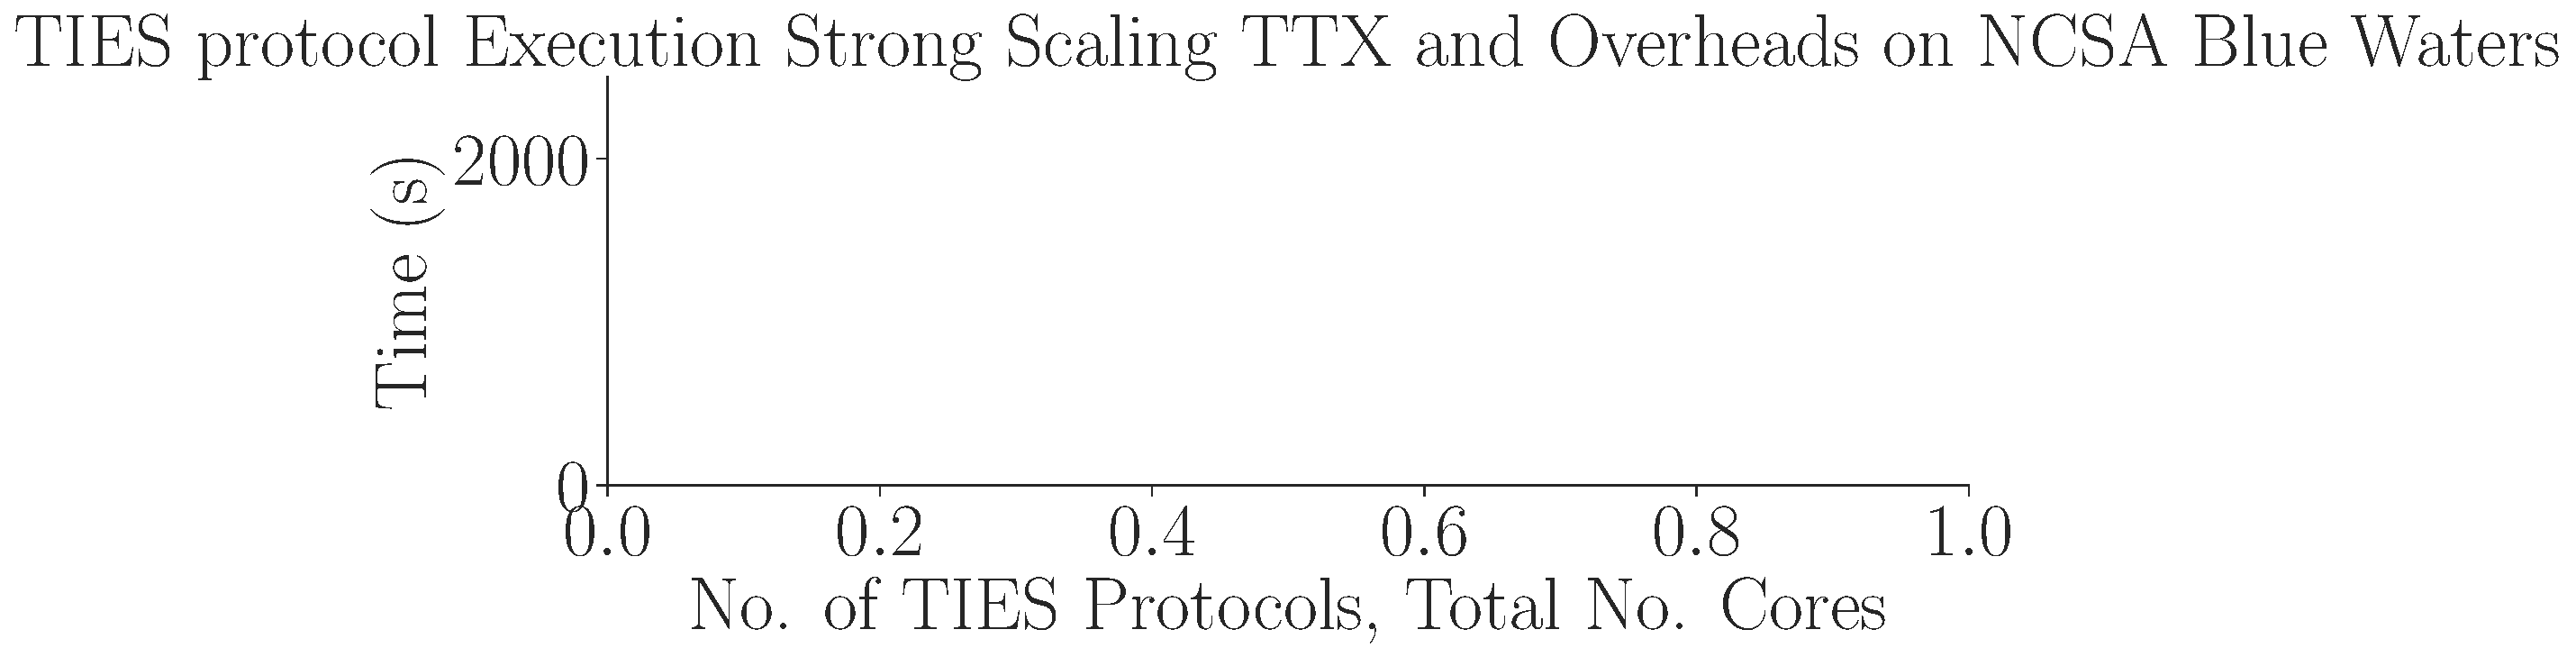
\includegraphics[width=\columnwidth]{figures/ties_ss_pseudo.pdf}
    \caption{Strong scaling properties of HTBAC using TIES protocols. We
    investigate the strong scaling of HTBAC with a fixed number of protocol
    instances while varying the amount resources. Overheads of HTBAC and
    runtime overhead (left) and \(TTX\) (right) for experimental
    configurations investigating the strong scaling of TIES.}
\label{fig:strong_scaling_TIES}
\end{figure}


(introduce experiment showing difference in overhead for EoP and PoE)


%----------------------------------------------------------------------------
\subsubsection{Validation Experiment}

\mtnote{Validation ExperimentS?}

HTBAC automates the process of calculating the binding affinity of
protein-ligand complexes from reading the input to analyzing the final
results. In order to validate the correctness of the results, we have devised
a set of experiments. These experiments are vital to gain confidence in the
algorithm and to prove that it is indeed calculating the correct values.

The validation experiments were based on the original study of Wan et. al.
\cite{Wan2017brd4}. We selected a subset of the protein ligand systems that
were the subject of that study: they are the ligand transformations 3 to 1,
4, and 7. We then performed a full simulation on all 3 systems and calculated
the binding affinity (see Table~\ref{tab:exp2}) using HTBAC.

The results show that all three $\Delta \Delta$G values are within error bars
of the original study, reinforcing the fact that HTBAC has indeed correctly
implemented the complex workflow of TIES.

\begin{table}
  \centering
  \caption{Comparison of the calculated binding free energies using HTBAC,
  from the original study by Wan et. al and experimental data. In principle,
  the two theoretical studies used the same protocol. This experiment proved
  that HTBAC implemented TIES correctly, as the calculated values are either
  the same or within error bar of the original study. All values are in
  \textbf{kcal mol\textsuperscript{-1}}.}
  % \begin{tabular}{l@{\hskip 1in}r@{\hskip 0.2in}r@{\hskip 0.2in}r}
  \begin{tabular}{lrrr}
    \toprule
    System & HTBAC & Wan et. al & Experiment \\
    \midrule
    BRD4 \textbf{3 to 1} & \num{0.39 +- 0.10} &   \num{0.41 +- 0.04} &  \num{0.3 +- 0.09} \\
    BRD4 \textbf{3 to 4} & \num{0.02 +- 0.12} &   \num{0.01 +- 0.06} &  \num{0.0 +- 0.13} \\
    BRD4 \textbf{3 to 7} & \num{-0.88 +- 0.17} &  \num{-0.90 +- 0.08} & \num{-1.3 +- 0.11} \\
    \bottomrule
  \end{tabular}
  \label{tab:exp2}
\end{table}

%----------------------------------------------------------------------------
\subsubsection{Adaptive Experiments}

The TIES workflow can benefit from an adaptive execution environment to
improve the efficiency and accuracy of result. In \emph{adaptive experiments}
we implemented the adaptive quadrature algorithm specifically customized for
biosimulations.

In the adaptive workflow, over the course of a protocol instance we alter the
number of $\lambda$ windows being simulated. The position of new $\lambda$
windows depends on the estimated error of the integral measured between
adjacent windows. Increasing the number of $\lambda$ windows in regions of
rapid change will increase the accuracy of the overall integral to a greater
degree than an arbitrarily placed window. In order to adaptively add lambda
windows, we need access to the $\partial U/\partial\lambda$ values during
runtime. Therefore, we break down the single production simulation stage (S4)
from the nonadaptive workflow into multiple smaller stages, each running for
1 ns. Once each simulation is complete within a stage a decision is made
about whether more $\lambda$ windows are required, and if so where they
should be placed.

We start out the simulation with 5 replicas of \emph{3} equally spaced
$\lambda$ windows, and equilibrate them. Then we repeatedly execute shorter
production simulations followed by an analysis phase which determines where
to place new lambda windows. This procedure is repeated until convergence, at
which point all concurrent simulation are terminated. We define convergence
as the point in the production-analysis loop at which a desired error
threshold is reached.

The success of this algorithm is determined by the decision where additional
$\lambda$ windows should be introduced. In adaptive quadrature, this decision
is made by calculating an error estimate on the integral and comparing this
to a threshold value. Due to the stochastic nature of biosimulations, it is
non-trivial to determine this error, and as a proof of concept we simplified
this decision to replicate pre-calculated results. In future studies we plan
to replace this with a dynamic decision process.

Inter-node communication introduces a constraint on the number of new lambda
windows that can be added at each iteration. To reduce the overhead of
inter-node communication, simulations must run on an integer number of nodes.
This means that the number of new $\lambda$ windows (i.e. the number of
simulations) \emph{has} to be either doubled or left unchanged. If the number
of window is doubled the nodes per simulation can be halved automatically.
Our prototype algorithm loops through the current $\lambda$ window pairs
until this criterion is reached, forcefully adding more if needed.


% I don't think we need this equation here, it's too trivial.
% \begin{flalign}
% L &= \{ x_i: x_i\in[0,1]\; and\; x_{i+1} = x_i + \delta \}, where\ \delta\ is\ 0.5.
% %&$$L=\{ x_i: x_i\in[0,1]\; and\; x_{i+1} = x_i + \delta \}$$%, where $\delta$ is $0.1$.
% \end{flalign}

% For every $\lambda$ window we initialize with five replicas therefore yielding a
% total of 15 tasks. We run 15 tasks for stages $S1$ through $S4.1$. Between
% stages $S4.1$ and $S4.3$ the number of $\lambda$ windows doubles
% for every stage, which doubles the total number of tasks. The last production
% simulation stage, $S4.4$, runs for the remaining 2 ns durations.

We introduce only a single degree of freedom relative to baseline ``non-
adaptive" experiments, thus our experiments implement adaptive change in the
$\lambda$ windows sampled and not the timing of execution. HTBAC provides the
functional capability to adaptively determine the time at which the $\lambda$
windows are chosen. However in this paper, we do not investigate the impact
of such adaptivity, as the objective is to determine the feasibility of
adaptive execution and resulting scientific merit of adaptive decision
making.

% \begin{figure}
%   \centering
%    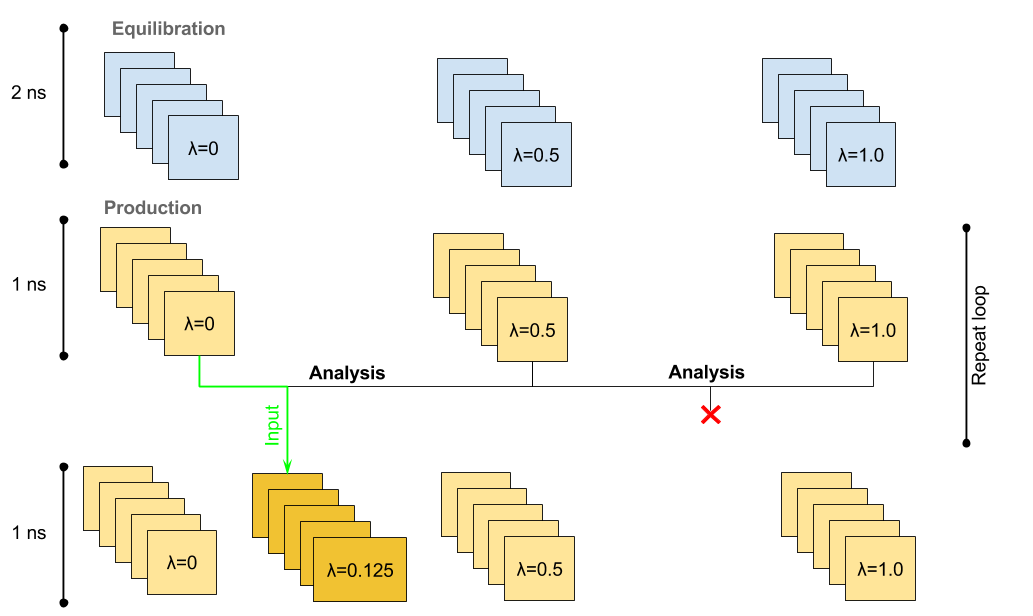
\includegraphics[width=\columnwidth]{figures/Adaptive_TIES_1.png}
%   \caption{Illustrating the adaptive workflow. After the 3 initial lambda 
%   windows are equilibrated, the first production stage starts. 
%   This is followed by analysis at every lambda interval, to decide whether 
%   to add a new window in the middle. The production-analysis is repeated 
%   for 4 production steps in our implementation, not shown here.}
% \label{fig:adaptive_TIES}
% \end{figure}

\begin{figure}
  \centering
    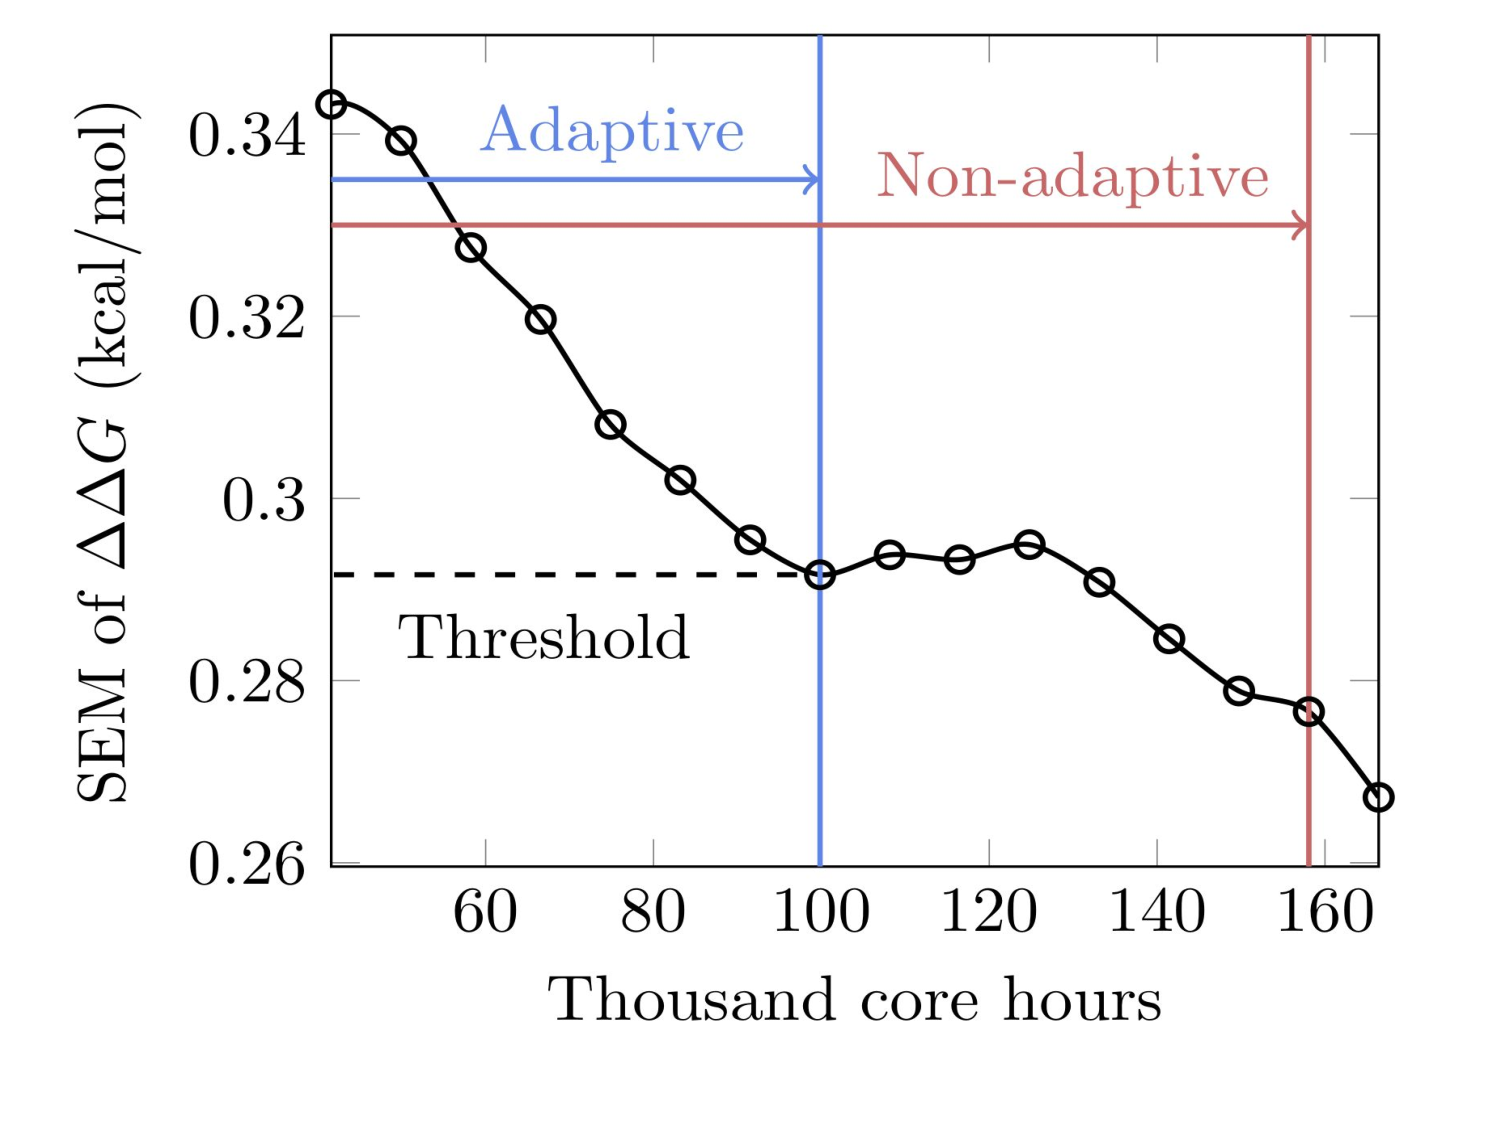
\includegraphics[width=\columnwidth]{figures/adaptive_vs_nonadaptive_pseudo.pdf}
    \caption{Illustrating the adaptive vs. non-adaptive workflow given the
    same number of core hours}
\label{fig:adaptive_vs_nonadaptive_TIES}
\end{figure}

% ---------------------------------------------------------------------------
\subsubsection{Adaptive Quadrature Experiments Results}

\mtnote{Should this be Results as a whole? Or are we missing the results for
all the others?}

One way to visualize the adaptivity in this experiment is to plot the
function and integral approximations at every iteration.
Figure~\ref{fig:adapt} shows how the value of $\Delta$G (i.e. the integral of
the function) for test system \textbf{3 to 7} improves as the algorithm
places more lambda windows. It is imporant to note, that the new points are
decided {\it a priori} for reasons discussed above but this is opaque to the
algorithm. This is a proof that we have the adaptive capabilities and which
pave the way for more advanced biosimulation algorithms.

\begin{figure}
  \centering
\begin{tikzpicture}
\begin{axis}[
  xlabel=$\lambda$,
  ylabel=$\frac{dU}{d\lambda}$,
  xmin=0,
  xmax=1,
  legend pos=north west,
  grid=both,
  ]
  \addplot+[name path=alch_1, mark size=1pt, mark=*, color=blue] table [x=lambda, y=p1v]{alch_1.csv};
  \addlegendentry{Iteration 1: Initial};

  \addplot+[name path=alch_2, mark size=1pt, mark=*, color=red] table [x=lambda, y=p1v]{alch_2.csv};
  \addlegendentry{Iteration 2: Increase};

  \addplot+[name path=alch_3, mark size=1pt, mark=*, color=brown] table [x=lambda, y=p1v]{alch_3.csv};
  \addlegendentry{Iteration 3: Optimized};

  \addplot+[name path=alch_4, mark size=1pt, mark=*, color=black] table [x=lambda, y=p1v]{alch_4.csv};
  \addlegendentry{Iteration 4: Sampling};

  \addplot[name path=line, draw=none] {0};

  \addplot fill between[
    of = alch_1 and line,
    split,
    every even segment/.style = {pattern color=blue!50, pattern=vertical lines},
    every odd segment/.style = {pattern color=blue!50, pattern=vertical lines},
    soft clip={domain=0:1},
  ];

  \addplot fill between[
    of = alch_2 and line,
    split,
    every even segment/.style = {pattern color=red!50, pattern=horizontal lines},
    every odd segment/.style = {pattern color=red!50, pattern=horizontal lines},
    soft clip={domain=0:1},
  ];

  \addplot fill between[
    of = alch_3 and line,
    split,
    every even segment/.style = {pattern color=brown!50, pattern=north east lines},
    every odd segment/.style = {pattern color=brown!50, pattern=north east lines},
    soft clip={domain=0:1},
  ];

\end{axis}
\end{tikzpicture}
\caption{Approximating the intergral under the curve, hence calculating
$\Delta$G. The adaptive algorithm reevaluates the efficiency of the lambda
window mesh after every \SI{1}{\nano\second} and makes a decision whether to
place more lambda windows inside certain ranges. As we iterate every 1 ns,
the integral approximation becomes more accurate.}
\label{fig:adapt}
\end{figure}
